\subsection{Implicit Differentiation}\label{subsec:implicit-differentiation}

\begin{center}
    Explained in the following example.
\end{center}

\begin{gather*}
    \frac{dy}{dx}(x^2+y^2+y=25)\\
    2x+2yy'+y'=0\\
    y'(2y+1)=-2x\\
    \frac{dy}{dx}=y'=\frac{-2x}{2y+1}\\
\end{gather*}

\subsection{Related Rates}

\subsubsection{Shadow Problem}

\begin{center}
    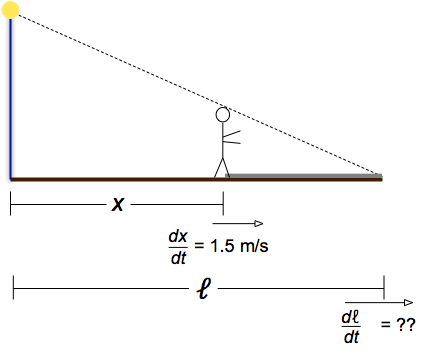
\includegraphics[scale=0.5]{figures/rr_shadow_ov.png}
\end{center}

A 1.8-meter tall man walks away from a 6.0-meter lamp post at the rate of 1.5 m/s. 
The light at the top of the post casts a shadow in front of the man. 
How fast is the “head” of his shadow moving along the ground?

\vspace{5mm} 

Must find $\frac{dl}{dt}$. 
The strategy is to use similar triangles to relate $x$ and $l$.

\begin{center}
    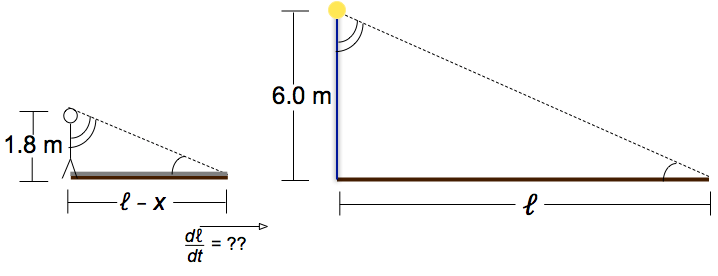
\includegraphics[scale=0.5]{figures/rr_shadow_str.png}
\end{center}

\begin{gather*}
    \frac{l-x}{l}=\frac{1.8}{6.0}\\
    l-x=0.3l\\
    x-l=0.30l\\
    x=0.7l\\
\end{gather*}

\vspace{5mm}

\begin{gather*}
    0.7\frac{dl}{dt}=\frac{dx}{dt}\\
    \frac{dl}{dt}=\frac{1.5}{0.7}\\
    \frac{dl}{dt}=2.1 \frac{m}{s}\\
\end{gather*}

\subsubsection{Trough Problem}

\begin{center}
    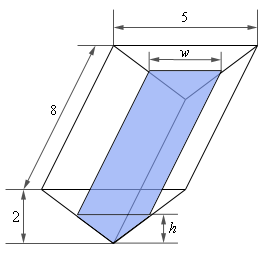
\includegraphics[scale=.5]{figures/rr_trough.png}
\end{center}

A trough of water is 8 meters in length and its ends are in the shape of isosceles triangles whose width is 5 meters and height is 2 meters.
If water is being pumped in at a constant rate of 6 $m^3$/sec, 
at what rate is the height of the water changing when the water has a height of 120 cm? 
At what rate is the width of the water changing when the water has a height of 120cm?

\vspace{5mm}

It is known that $V'=6 m^3$/sec.
Need $h'$ when $h=1.2$.

\vspace{5mm}

The volume of the water in the tank is given by:

\begin{gather*}
    V=\frac{1}{2}base\times{height}\times{depth}\\
    =\frac{1}{2}hw(8)\\
    =4hw\\
\end{gather*}

Need to eliminate $w$ as target is $h'$.
Using similar triangles.

\begin{gather*}
    \frac{w}{5}=\frac{h}{2} \Rightarrow w=\frac{5h}{2} \Rightarrow V=10h^2\\
    V'=20hh' \Rightarrow 6=20(1.2)h' \Rightarrow h'=0.25m/sec\\
\end{gather*}

R.O.C of width can be found by manipulating similar triangles to get $V$ in terms of $w$ only.

\[h=\frac{2w}{5} \Rightarrow V=\frac{8w^2}{5}\]

Differentiate and substitute as before.

\subsection{L'Hopital's Rule}\label{subsec:l'hopital's-rule}

\subsubsection{Indeterminate Forms: $\frac{0}{0}$ or $\frac{\infty}{\infty}$}

\[\lim_{x\to{c}}\frac{f(x)}{g(x)}\]

Suppose that $f(x)=0$ and $g(x)=0$ and that $c \in \R$.

\[\lim_{x\to{c}}\frac{f(x)}{g(x)}=\lim_{x\to{c}}\frac{f'(x)}{g'(x)}\]

Process can be repeated.

\subsubsection{Indeterminate Forms: $\infty \cdot 0$ or $\infty - \infty$}

Requires that the limit be rewritten in fractional form for differentiation.

\begin{gather*}
    \lim_{x\to{0^+}}x\csc{x}\\
    x\csc{x}=\frac{x}{\sin{x}}\\
    \lim_{x\to{0}}\frac{x}{\sin{x}}=\frac{1}{\cos{x}}|_{0}=\frac{1}{1}=1\\
\end{gather*}

\subsubsection{Indeterminate Forms: $0^0$, $1^\infty$, or $\infty^0$}

Incorporates changes using logarithms in order to get limit in to the form
as shown before. 

\begin{gather*}
    L=\lim_{x\to{0^+}}x^x\\
    \ln{L}=x\ln{x} \Rightarrow -\infty \cdot 0\\
    \ln{L}=\lim_{x\to{0^+}}=\frac{\ln{x}}{\frac{1}{x}}=\frac{\frac{1}{x}}{\frac{-1}{x^2}}\\
    \ln{L}=\lim_{x\to{0^+}}-x=0\\
    e^{\ln{L}}=e^0\\
    L=1\\
\end{gather*}

Special example in the following form:

\[\lim_{x\to{c}}(d+\frac{a}{x})^{bx}=e^{ab}\]

\subsubsection{Limit Definition of Derivative}

In the form $f'(x)=\lim_{h\to{0}}\frac{f(x+h)-f(x)}{h}$, 
where the derivative is taken with respect to $h$.
By recognizing this form, the answer would be $\frac{d}{dx}f(x)$.